\mychapter{Esrtutura do Sistema}
\label{Cap:estruturaSistema}


A fim de atender aos objetivos desejados de maneira coerente ao que se observa nas instalações do laboratório, tem-se a necessidade de entender as mesmas para determinar uma forma de desenvolver o projeto posteriormente. Devido a isso, pode-se dizer que as instalações do Laboratório de Injeção do LAMP serviram como base para esse trabalho, visto que a partir delas, percebeu-se a necessidade da criação de um sistema supervisório e de interligar os elementos do projeto industrial. 

A fim de entender melhor a base do trabalho, esse capítulo apresenta inicialmente uma descrição dessas instalações e posteriormente, a descrição do sistema montado, considerando especificações técnicas, características, instrumentos e protocolos utilizados.

\section{Instalações do Laboratório}

O LAMP dispõe de um espaço de instalações físicas de uma planta do Laboratório de Monitoramento de Injeção com o objetivo de realizar ensaios de medição de vazão. Um diagrama das instalações do laboratório pode ser observado na Figura \ref{fig:Planta}. A figura consiste em uma simplificação da planta, ilustrando apenas componentes essenciais para o entendimento do sistema.



\begin{figure}[h!]
  \center
  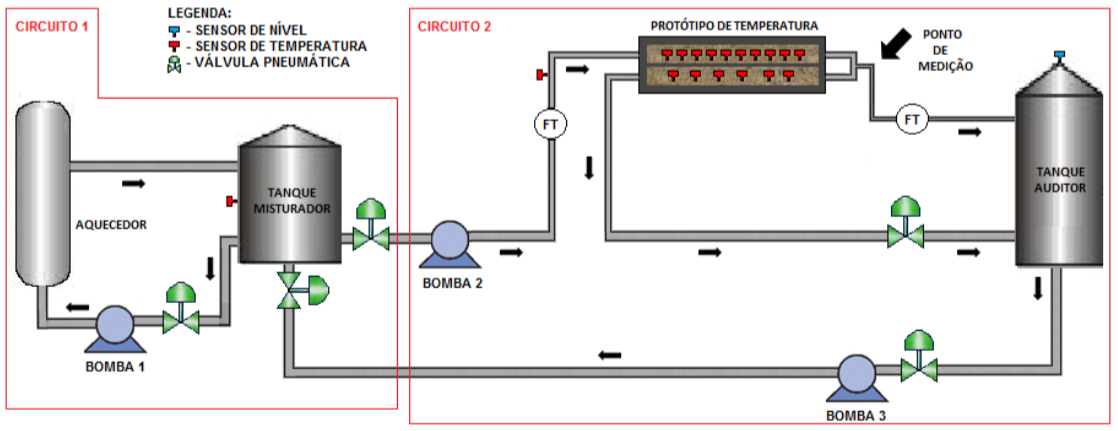
\includegraphics[scale=0.6]{Planta.png}
  \label{fig:Planta}
  \caption{Ilustração simplificada das Instalações do Laboratório de Monitoramento de Injeção.}
\end{figure}


O protótipo é composto pelos seguintes componentes:

\begin{itemize}
    \item Dois tanques de armazenamento de líquido
    \item Aquecedor: cilindro de aquecimento de água
    \item 5 Válvulas de acionamento pneumático
    \item 3 Bombas de deslocamento positivo
    \item 18 Sensores de temperatura
    \item 2 Sensores de nível
    \item 2 Sensores de vazão
    \item 4 Chaves de nível
\end{itemize}


O sistema é operado através de dois circuitos: o primeiro circuito é responsável por aquecer a água armazenada inicialmente no tanque misturador, enquanto o segundo irá transferir a água aquecida para caixotes os quais simulam a zona de injeção. Desse modo, para que o sistema funcione corretamente, a água deve estar contida no sistema de forma que as tubulações devem estar afogadas e os tanques devem conter água também.

Um sistema de aquecimento também é contido na planta. Este é responsável por fornecer energia térmica à água utilizada nos ensaios e é composto por controladores, sensores e atuadores em uma malha fechada. Sendo assim, é imprescindível que haja uma comunicação entre esses três componentes para que o sistema funcione corretamente.

\subsection{Modo de operação do circuito 1}

Para que a planta entre em operação, a válvula pneumática de saída do tanque misturador é aberta, enquanto as outras estão fechadas. Devido à ação da bomba 1, a água circula através do aquecedor, aumentando sua temperatura e retornando ao tanque misturador. Esse processo é executado em um ciclo fechado até que a temperatura desejada para a água seja atingida. 

Para que esse circuito funcione de maneira satisfatória, os dados da temperatura da água devem ser medidos e a grandeza deve ser controlada. Para isso, um controlador dedicado é responsável por controlar o acionamento do aquecedor através das informações advindas do sensor de temperatura conectado ao tanque misturador. O controlador de processos utilizado para essa finalidade é o da fabricante NOVUS modelo N2000 que será discutido mais adiante neste capítulo.

\subsection{Modo de operação do circuito 2}

No momento em que a temperatura desejada para os testes é alcançada, a bomba 2 é acionada e a água aquecida é enviada ao circuito 2, responsável pela medição dos parâmetros de temperatura e vazão, de forma a simular um sistema petrolífero real. 

Nesse circuito, a água segue para uma tubulação que simula um poço de petróleo, enterrada dentro de dois caixotes cobertos de areia. Nessa tubulação, 16 sensores te temperatura foram distribuídos com o objetivo de identificar a variação térmica ao longo da coluna de injeção, advinda da troca de calor entre o fluido injetado e o solo. A análise de vazão é realizada no ponto de medição descrito na Figura \ref{fig:Planta}. Nesse trecho é feito o controle de vazão variando-se a vazão nas derivações dos tubos de 1" e 2" que se encontram nesse ponto. Dessa forma, um perfil de temperaturas é obtido antes e outro depois do ponto de medição de vazão. Através da variação forçada da vazão do sistema, é possível comprovar e analisar o desenvolvimento teórico do projeto, pois dessa forma pode-se obter perfis de temperaturas para variadas condições de trabalho do protótipo.

Após a passagem pelo protótipo de temperatura, o líquido é armazenado temporariamente no tanque auditor. Será configurado um nível mínimo de fluido presente no tanque misturador, que quando atingido, a bomba 3 será acionada e o fluido presente no tanque auditor será bombeado para o misturador, completando o ciclo do segundo circuito.

\section{Especificações teóricas}

Pode-se afirmar que o sistema descrito no item 2.1 serve como base para o desenvolvimento desse trabalho pois para que ocorra a captação dos dados dos elementos de instrumentação descritos anteriormente, é necessária a comunicação desses ao sistema supervisório que será desenvolvido. Em intermédio a essa comunicação, é utilizado um Controlador Lógico Programável (CLP). Um CLP é um equipamento eletrônico digital composto com hardware e software utilizado em sistemas industriais, capaz de manipular elementos desses sistemas.

Esse tipo de controlador é utilizado em larga escala na indústria para o controle de diversos tipos de sistemas pois atendem a requisitos de hardware e software aptos para serem utilizados em ambientes industriais. Neste sentido, muitos CLPs possuem sistemas operacionais de tempo real, fator de extrema importância para controlar processos de alto risco, e hardware capaz de suportar possíveis variações de pressão, temperatura e umidade, além de a maioria deles possuir uma arquitetura compacta, o que facilita o deslocamento e instalação do controlador. Outra grande vantagem da utilização de CLPs na indústria é a sua capacidade e relativa facilidade de comunicação com outros elementos da malha industrial e com sistemas supervisórios.

Sistemas de Supervisão e Aquisição de Dados (SCADA) são sistemas utilizados amplamente na indústria para controle supervisório e aquisição de dados de processos industriais. Como o próprio nome indica, esses sistemas são focados no nível de supervisão de processos, sendo puramente softwares posicionados acima dos hardwares da interface industrial que podem se comunicar com CLPs ou outros hardwares \cite{daneels1999scada} para uma melhor visualização e manipulação da malha industrial a ser controlada. O sistema SCADA necessário para os projetos futuros a esse deve, em termos simplificados, comportar uma representação visual de todo o sistema físico das instalações do LAMP, captar os dados dos elementos de instrumentação e realizar possíveis controles da planta industrial de modo remoto. Durante esse trabalho, foi proposto um sistema SCADA somente para testes de comunicação e captação de parâmetros que é descrito com mais detalhes no capítulo 3 desse trabalho.

Existem diversos tipos de CLPs que variam de acordo com cada fabricante. No projeto realizado, foi utilizado um controlador lógico programável da WEG modelo TPW-03 60HT-A e um controlador universal de processos da NOVUS modelo N2000. Para desenvolvimento do sistema supervisório, utilizou-se o software Elipse SCADA. O controlador lógico da WEG foi utilizado pois ele possui uma quantidade satisfatória de entradas e saídas digitais e também dispõe de módulos de expansões, dentre eles o modelo 8AD, o qual fornece entradas analógicas, que possibilitam a leitura dos sensores que irão atuar no projeto. O Elipse SCADA, por sua vez, mostra-se um software bastante eficiente para controle supervisório, de fácil manipulação e de maior familiaridade por parte dos engenheiros do LAMP.

\section{Instrumentos Utilizados}

O trabalho aqui descrito foi realizado nos laboratórios do LAMP e os instrumentos utilizados foram:

\begin{itemize}
    \item 2 sensores de temperatura PT100
    \item 1 CLP da WEG modelo TPW-03 60HT-A
    \item 1 módulo de expansão do tipo 8AD 
    \item 1 fonte de alimentação ($24V$)
    \item 1 controlador de processos da NOVUS, modelo N2000
    \item 2 computadores para alojamento do sistema supervisório, realização de pesquisas e testes
\end{itemize}


O ambiente de trabalho é observado na Figura 2.2.%\ref{fig:Ambiente} 

\begin{figure}[h!]
  \center
  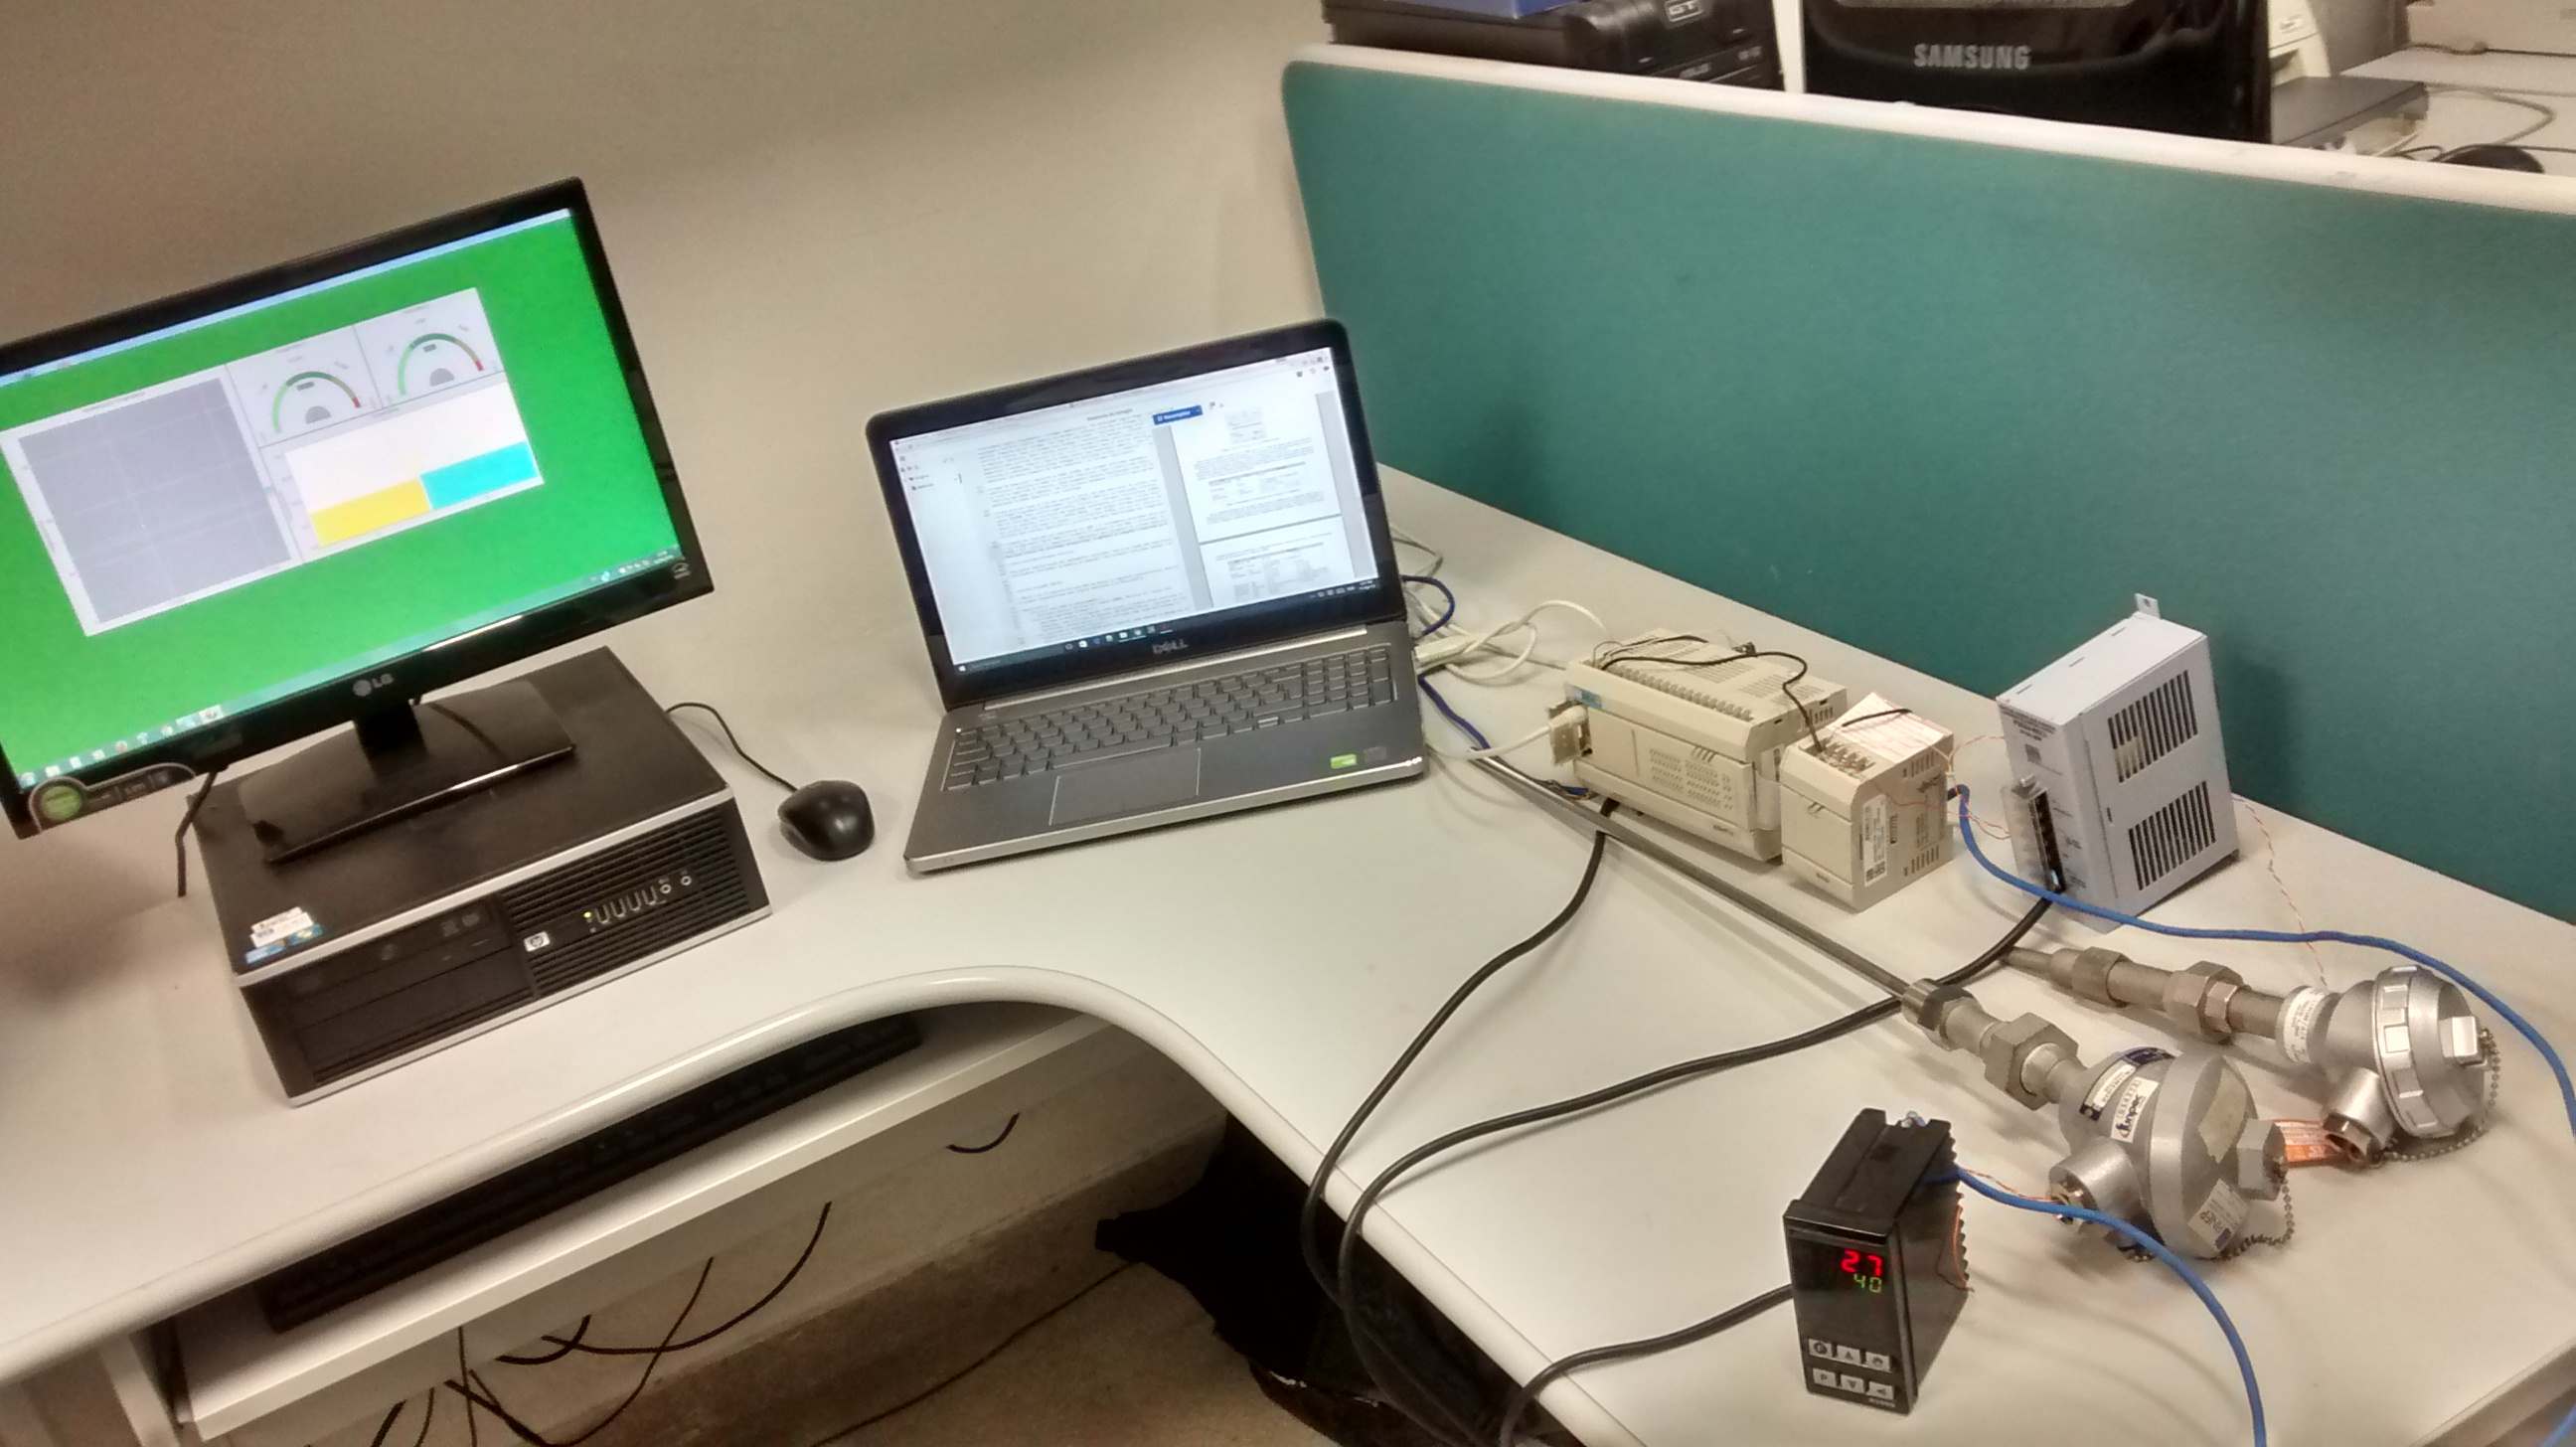
\includegraphics[scale=0.15]{Ambiente.jpg}
  \label{fig:Ambiente}
  \caption{Ambiente de Trabalho.}
\end{figure}


\section{Características e Especificações Técnicas}

Para melhor familiarização dos equipamentos utilizados, tem-se um resumo das especificações técnicas dos controladores, dos módulos de expansão, dos softwares e protocolos utilizados no trabalho.

\subsection{Sensores PT100}

Como já mencionado anteriormente, para obter os padrões de temperatura do líquido que passa pelo sistema do laboratório de injeção no LAMP, são necessários 18 sensores de temperatura. Esses sensores são do tipo PT100 (Figura 2.3), com transmissores de modelo TR321 da fabricante Salcas. Neste trabalho, utilizou-se dois desses sensores para que os testes realizados sejam condizentes com uma futura implementação do sistema final no laboratório.

\begin{figure}[h!]
  \center
  \label{fig:Pt100}
  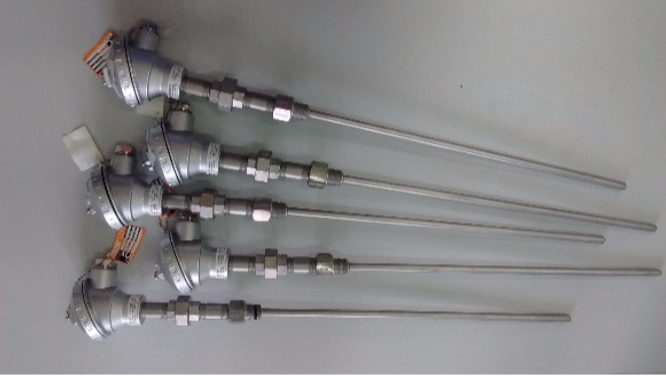
\includegraphics[scale=0.8]{Pt100.png}
  \caption{Sensores de temperatura PT100.}
\end{figure}

O funcionamento desses sensores baseia-se na variação da resistência ôhmica em relação à temperatura. Seu elemento sensor é composto por platina com grande grau de pureza e encapsulado em bulbos de vidro ou cerâmica, o que permite uma medição padrão de termorresistência entre -200 e 650ºC \cite{salcas2015site}. Por essas características, esses sensores são um dos mais utilizados em processos industriais. Além disso, as termorresistências são totalmente customizáveis, sendo possível alterar o limite de operação do sensor para que se obtenha medidas mais precisas dependendo da aplicação. Nesse caso, como os sinais gerados pelo transmissor estão na faixa de 4 à 20 mA, o limite de medição pode ser configurado no transmissor para que o valor mínimo/máximo de corrente gerado corresponda a um valor de temperatura próximo ao mínimo/máximo em que o sistema industrial estará sujeito.

Para a aplicação em desenvolvimento nas instalações do LAMP, a água estará sujeita a temperaturas que variam entre aproximadamente 25 e 65ºC, logo, é mais eficiente definir a faixa de operação do transmissor entre esses dois valores para que seja obtida uma melhor resolução de leitura das variáveis. Essa alteração é feita através do software \textit{TxConfig II}, disponibilizado pelo fabricante.



\subsection{WEG TPW-03}

O TPW-03 é um CLP desenvolvido pela empresa WEG Automação S.A. que possui as seguintes características, descritas no manual de instalação do produto disponibilizado pelo próprio fabricante \cite{weg2010manualinstalacao}:

\begin{itemize}
    \item Alta velocidade de processamento:\\
        Instruções básicas: $0.31\mu s$ / passos (ANDB), $0.45\mu s$ / passos (LD)
    \item Grande capacidade de memória:\\
        Capacidade de memória do programa: 4k a 16k passos. O produto possui instruções de aplicação básicas e integradas, como instruções de operação, ADD/SUB/MUL/DIV…etc. instruções de trigonometria como SIN/COS/TAN…, entrada matriz, e outras instruções como saída para display de 7 segmentos e PID.
    \item Capacidade de expansão flexível:\\
        Unidades básicas: 14/20/30/40/60 pontos digitais, pode expandir no máximo até 124 pontos digitais e 8/2 (12 bits) entrada/saída analógica.
    \item 3 portas de comunicação e 3 funções de comunicação são disponíveis no modelo avançado.
    \item Conexão com Computador:\\
        Um computador pode controlar até 255 TPW-03s.
    \item Conexão de Dados: \\
        O TPW-03 Mestre pode comunicar com até 15 TPW-03 Escravos. Cada CLP tem disponível para troca de dados 64 Bits e 8 Words.
    \item E/S Remota:\\
        O TPW-03 Mestre pode controlar as E/Ss de até 4 outros TPW-03 Escravos.
    \item Compatível com Modbus:\\
        O Protocolo Modbus está desenvolvido no TPW-03. Ideal para comunicação com Inversores e IHMs.
    \item RTC, PWM, dois VR’s (potenciômetros), memória flash e capacidade de expansão de pontos digitais e analógicos.
    \item Saída de pulso de alta velocidade de 100KHz que pode controlar um servo controlador.
    \item Contador de alta velocidade:\\
        O contador pode trabalhar um ou dois canais e como entrada de interrupção, sendo que no modo contagem com um canal, sua freqüência máxima é de 100KHz.
    \item Fácil manutenção e instalação uma vez que os blocos de terminais são plugáveis.
    \item O TPW-03 pode ser programado nas linguagens Ladder e Lista de Instruções.
    \item O Firmware pode ser atualizado diretamente via PC.
\end{itemize}

O LAMP dispõe de CLPs de modelo de modulo básico TPW-03 60HT-A, o qual possui uma alimentação AC 100 - 240V, 36 entradas digitais e 24 saídas digitais do tipo transistor. Além disso, foram utilizados módulos de expansão modelo 8AD (expansão analógica), que dispõem de oito entradas analógicas, o que permite a captação de dados de sensores.

O TPW-03 possui um software de programação em LADDER próprio, o TPW03-PCLINK. Esse software foi utilizado para configurar os parâmetros de comunicação do CLP com outros controladores e com o Elipse SCADA. Essa comunicação será comentada mais adiante neste trabalho.

\subsection{NOVUS N2000}

O controlador universal da NOVUS modelo N2000 possui os seguintes detalhes técnicos \cite{novus2014folheto}:
\begin{itemize}

    \item Aceita termopares: J, K, T, N, R, S, E, B; PT100, 4-20 mA, 0-50 mV, 0-5 Vcc, 0-10 V
    \item Saídas: relé 3 A / 250 Vca, linear 4-20 mA e pulso lógico para relés de estado sólido 
    \item Alarmes: 4 relés na versão básica 
    \item Até 2 alarmes temporizados de 0 a 6500s 
    \item Resolução na medida: 12000 níveis 
    \item Indicação de decimais nas medições de temperatura
    \item Proteção da configuração por senha de acesso
    \item Interface USB 2.0, classe CDC, protocolo Modbus RTU
    \item Fonte 24 Vcc para excitar transmissores
    \item Amostragem: 5 medidas por segundo.
    \item Alimentação: 
    - 100 a 240 Vca/cc 
    - 12 a 24 Vcc / 24 Vca 
    \item Retransmissão da PV ou SP em 0 a 20 mA ou 4 a 20 mA
    \item Função Automático/Manual, transferência \textit{bumpless}
    \item Entrada de SetPoint remoto
    \item Função LBD (Loop Break Detection)
    \item Entrada Digital
    \item Função saída segura
    \item Soft-start programável (0 a 9999 seg.)
    \item Rampas e Patamares: 7 programas de 7 segmentos cada, podendo ser concatenados até formar um programa de 49 segments. Todos os segmentos podem ser associados eventos.
    \item Auto-sintonia dos parâmetros PID
    \item Teclas em silicone 
    \item Painel frontal: IP65, Policarbonato UL94 V-2
    \item Formato 48 x 96 x 92 mm
    \item Certificações CE e UL
    
\end{itemize}

Tem-se uma amostra desse controlador disponível no laboratório e o mesmo foi utilizado a fim de se comunicar com o sistema supervisório e com o TPW-03 através de comunicação serial RS485 com protocolo Modbus RTU. Esse controlador possui a vantagem de ser leve e de pequenas dimensões, além de dispor de uma fácil programação de seus parâmetros, sendo estes configuráveis através de suas teclas, no próprio aparelho, não necessitando de um ambiente de programação. Além disso, esse controlador possui entradas analógicas, que permitem também a leitura de sensores do tipo PT100, que são utilizados no trabalho.


\subsection{Elipse SCADA}

O Elipse SCADA é um software de monitoramento e programação de processos muito utilizado em linhas de produção e ambientes industriais. Nele os dados dos sistemas podem ser apresentados em tempo real de forma gráfica \cite{elipse2015manual}, o que permite uma análise eficiente e respostas rápidas. O programa conta com uma ferramenta denominada \textit{Organizer} que permite uma organização das variáveis e propriedades do sistema de forma amigável, auxiliando na organização e manipulação dos parâmetros do sistema através de \textit{displays}, botões, gráficos, etc. Outro fator primordial para a utilização desse software no projeto aqui descrito, é a possibilidade de integrar o mesmo a controladores e unidades remotas de diversas maneiras, dentre elas, via protocolo Modbus, com comunicação RS485 ou Ethernet.

\subsection{Protocolo Modbus}

O Modbus é um tipo de protocolo de comunicação, proposto pela Modicon Corporation. Esse protocolo define uma estrutura de mensagem que diferentes controladores podem reconhecer e utilizar independente do tipo de rede em que eles estão conectados. Ele descreve o processo que um controlador utiliza para requisitar acesso a outro dispositivo, como ele vai responder à pedidos de outros dispositivos e como erros serão detectados e reportados. Além disso, o protocolo estabelece um formato comum de \textit{layout} e conteúdos de campos mensagem \cite{modbus1996manual}.

Em uma rede Modbus, o protocolo determina como cada controlador saberá o endereço de cada dispositivo, reconhecer a mensagem adereçada à ele, determinar o tipo de ação que será tomada e extrair o dado ou outra informação contida na mensagem. Se uma resposta é requisitada, o controlador vai construir a mensagem de resposta e mandar utilizando o próprio protocolo Modbus\cite{modbus1996manual}.

Os controladores da rede Modbus utilizam uma comunicação mestre-escravo, na qual apenas um dispositivo (o mestre) pode iniciar a transmissão dos dados por meio de uma requisição aos outros dispositivos (escravos). Os escravos, respondem enviando o dado requisitado pelo mestre ou realizando a ação que o dispositivo mestre desejou. No trabalho aqui realizado, o dispositivo mestre da rede de comunicação montada é o PC, o qual contém o processador \textit{host} da aplicação feita no Elipse SCADA. Os escravos correspondem ao CLP TPW-03 e ao controlador de processos N2000.

O mestre pode tanto adereçar mensagens a escravos individuais ou em \textit{broadcast}, para todos os escravos. Os outros dispositivos retornam a mensagem de resposta às requisições do mestre de forma individual. 

A forma com que o protocolo estabelece o formato de requisição do mestre se dá por indicar ao mestre o endereço do dispositivo ao qual ele deseja se comunicar, o código da função que define a ação a ser executada, algum possível dado a ser enviado e um campo de checagem de erro. A mensagem de resposta do escravo também é construída utilizando o mesmo protocolo. Ela contém campos confirmando a ação tomada, qualquer dado a ser retornado e um campo de checagem de erro. Se algum erro tiver ocorrido no recebimento da mensagem, ou se o escravo for incapaz de realizar a ação requisitada, o mesmo construirá uma mensagem de erro e enviará como resposta. A Figura 2.4 demonstra um esquema da comunicação entre um dispositivo mestre e um escravo.

\begin{figure}[h!]
  \center
  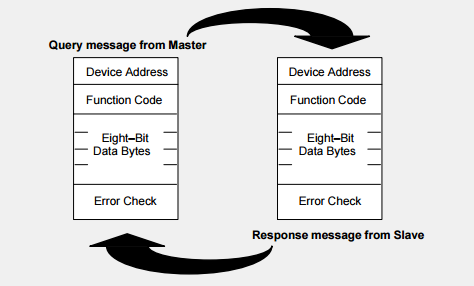
\includegraphics[scale=1.0]{QueryResponse.png}
  \label{fig:QueryResponse}
  \caption{Requisição-resposta entre mestre e escravo.}\cite{modbus1996manual}
\end{figure}
\subsubsection{Modos de Operação}

Uma rede Modbus padrão pode operar segundo dois modos de transmissão: ASCII ou RTU. Esses modos definem como a informação será contida e decodificada nos campos de mensagem. Quando os controladores são dispostos a se comunicar utilizando o modo ASCII \textit{(American Standard Code for Information Interchange)}, cada byte em uma mensagem é enviado como dois caracteres ASCII. A maior vantagem desse modo é que ele permite que intervalos de cerca de um segundo entre caracteres ocorram sem causar um erro. A Tabela \ref{tab:ASCII} demonstra o formato de 1 byte em operação no modo ASCII.

\begin{table}[]
\centering
\resizebox{\textwidth}{!}{%
\begin{tabular}{|c|c|}
\hline
 & \cellcolor[HTML]{C0C0C0}Modo ASCI \\ \hline
\cellcolor[HTML]{C0C0C0}Codificação & \begin{tabular}[c]{@{}c@{}}Hexadecimal, caracteres ASCII 0–9, A–F\\ Um caracter hexadecimal contido em cada caracter ASCII da mensagem\end{tabular} \\ \hline
\cellcolor[HTML]{C0C0C0}Bits por Byte & \begin{tabular}[c]{@{}c@{}}1 bit de início \\ 7 bits de dados\\ 1 bit de paridade; nenhum bit caso sem paridade\\ 1 bit de parada, se paridade é usada; 2 bits caso sem paridade\end{tabular} \\ \hline
\cellcolor[HTML]{C0C0C0}Checagem de Erro & Longitudinal Redundancy Check (LRC) \\ \hline
\end{tabular}%
}
\caption{Formato de Byte no Modo ASCII}
\label{tab:ASCII}
\end{table}


No modo de operação RTU \textit{(Remote Terminal Unit)}, cada byte (8 bits) presente em uma mensagem é composto por dois conjuntos de 4 bits de caracteres hexadecimais. A maior vantagem desse modo é que por haver uma maior densidade de caracteres em uma mensagem, há uma maior taxa de transferência neste com relação ao modo ASCII (considerando uma mesma taxa de transmissão). Devido a essas vantagens, 
neste trabalho, optou-se por utilizar o protocolo Modbus em modo RTU. Neste modo, cada mensagem deve ser transmitida em um fluxo contínuo de caracteres. A Tabela \ref{tab:RTU} demonstra o formato de 1 byte no modo de operação RTU.

\begin{table}[]
\centering
\resizebox{\textwidth}{!}{%
\begin{tabular}{|c|c|}
\hline
 & \cellcolor[HTML]{C0C0C0}Modo RTU \\ \hline
\cellcolor[HTML]{C0C0C0}Codificação & \begin{tabular}[c]{@{}c@{}}8–bit binário, hexadecimal 0–9, A–F\\  Dois caracteres hexadecimais contidos em cada campo de 8–bits da mesnesagem\end{tabular} \\ \hline
\cellcolor[HTML]{C0C0C0}Bits por Byte & \begin{tabular}[c]{@{}c@{}}1 bit de início\\  8 bits de dados\\  1 bit de paridade; nenhum bit caso sem paridade\\  1 bit de parada se paridade é usada; 2 bits caso sem paridade\end{tabular} \\ \hline
\cellcolor[HTML]{C0C0C0}Checagem de Erro & Cyclical Redundancy Check (CRC) \\ \hline
\end{tabular}%
}
\caption{Formato de Byte no Modo RTU}
\label{tab:RTU}
\end{table}

Na prática, se em um sistema Modbus, determinado equipamento escravo falha, ou é separado da rede, o mestre pode identificar o equipamento falho e após o reparo, a rede pode ser conectada novamente automaticamente. Assim, pode-se dizer que o protocolo Modbus é confiável em relação à falhas desse tipo \cite{peng2008modbus}.

Além desses dois modos de operação em serial, existe também o protocolo Modbus/TCP, em que o controle de acesso ao meio se dá via CSMA-CD (em rede Ethernet) com o modelo cliente-servidor. Esse modo de operação não foi considerado nesse trabalho, visto que a comunicação serial mostrou-se suficiente para a aplicação desenvolvida.

%ZZZZZZZZZZZZZZZZZZZZZZZZZZZZZZZZZZZZZZZZZZZZZZZZZZZZZZZZZZZZZZZZZZZZZZZZZZZZZZZZZZ

